\chapter{Methoden} \label{chap:methoden}

\section{Phylogenetische Analyse} \label{sec:phylogenetische-analyse}

Für die phylogenetische Untersuchung der Flaviviridae-Familie wurden 458 vollständige Genomsequenzen aus öffentlichen Datenbanken wie GenBank extrahiert. \autocite{mifsudMappingGlycoproteinStructure2024}. Die Auswahl der Genomsequenzen erfolgte auf Basis von Vollständigkeit, Annotation und Homologie, um fehlerhafte oder unvollständige Daten auszuschließen.

Als phylogenetischer Marker diente das \gls{nsfive}-Gen, welches die RNA-abhängige RNA-Polymerase (\gls{rdrp}) kodiert. Dieses Gen ist aufgrund seiner universellen Verbreitung und hohen Konservierung innerhalb der Flaviviridae ideal geeignet, um evolutionäre Beziehungen aufzuzeigen \autocite{Koonin1991}. Die \gls{rdrp} ist zentral für die virale RNA-Replikation und steht daher unter starkem Selektionsdruck, was ihre Sequenzstabilität über verschiedene Gattungen hinweg erklärt. Gleichzeitig enthält das Gen auch hinreichend variable Regionen, um divergente evolutionäre Linien zu identifizieren \autocite{Nguyen2015}.

Die phylogenetische Analyse basiert auf einem \gls{msa}, welches mithilfe des Programms \gls{mafft} erstellt wurde \autocite{Katoh2013}. MAFFT kombiniert Fourier-Transformationen mit den Alignments, um homologe Regionen zu identifizieren. Diese Methode liefert robuste Alignments, selbst bei hochdivergenten Sequenzen. Die mathematische Grundlage der Fourier-Transformation, die für die Erkennung konservierter Sequenzmotive eingesetzt wird, ist im Anhang \ref{sec:mafft-mathematik} beschrieben. Alternativmodelle wie Clustal Omega oder MUSCLE sind hier nicht passend, aufgrund ihrer geringeren Sensitivität bei langen und hochvariablen Sequenzen \autocite{edgarMUSCLEMultipleSequence2004}.

Das resultierende \gls{msa} wurde zur Rekonstruktion eines phylogenetischen Baumes herangezogen. Hierbei wurde die Maximum-Likelihood-Methode angewandt, die eine probabilistische Modellierung der evolutionären Prozesse erlaubt \autocite{felsensteinEvolutionaryTreesDNA1981}. Diese Methode optimiert die Wahrscheinlichkeit der beobachteten Daten unter Berücksichtigung der zugrunde liegenden Topologie des phylogenetischen Baumes und eines Substitutionsmodells. Für diese Arbeit wurde das General Time Reversible-Modell mit invarianten Positionen und gamma-verteilter Rate-Heterogenität (\gls{gtrig}) gewählt, da es eine flexible Modellierung von Nukleotidsubstitutionen ermöglicht und besonders für komplexe phylogenetische Beziehungen geeignet ist \autocite{Tavare1986}.

Die mathematische Formulierung des \gls{gtrig}-Modells, einschließlich der Parameter für Substitutionsraten, stationäre Wahrscheinlichkeiten und die Gamma-Verteilung, ist im Anhang \ref{sec:maxlikelihood} näher erläutert. Dieses Modell berücksichtigt die Heterogenität der Substitutionsraten zwischen verschiedenen Sequenzpositionen, wodurch die Genauigkeit der phylogenetischen Topologie verbessert wird \autocite{yangMaximumLikelihoodPhylogenetic1994}.

Um die Robustheit der rekonstruierten Topologie zu gewährleisten, wurde ein Bootstrapping mit 1.000 Wiederholungen durchgeführt \autocite{Felsenstein1985}. Bootstrapping evaluiert die Stabilität der Baumknoten, indem es zufällige Resampling-Techniken auf das ursprüngliche Alignment anwendet und die resultierenden Bäume miteinander vergleicht. Hohe Bootstrap-Werte (>90 \%) bestätigen die Zuverlässigkeit der Hauptknoten und ermöglichen eine fundierte Klassifizierung der Hauptkladen innerhalb der Flaviviridae. Die spezifische Berechnung der Bootstrap-Werte sowie ihre Bedeutung für die Interpretation der phylogenetischen Ergebnisse sind im Anhang \ref{sec:maxlikelihood} beschrieben.

Der endgültige phylogenetische Baum wurde mithilfe von Programmen wie FigTree und iTOL visualisiert, um die Hauptkladen und deren evolutionäre Beziehungen zu verdeutlichen \autocite{letunicInteractiveTreeLife2021}. Der Baum zeigt eine klare Aufteilung in drei Hauptkladen: \textit{Flavivirus}, \textit{Pegivirus/Hepacivirus} und \textit{Pestivirus/Jingmenvirus/LGFs}, die durch signifikante Unterschiede in Sequenz- und Strukturmerkmalen gekennzeichnet sind (s.\ref{fig:figure1-orginal}).

\section{Proteinstrukturvorhersage: ColabFold und ESMFold} \label{sec:colabfold-esmfold}

Die dreidimensionalen Strukturen der Glycoproteine der Flaviviridae wurden mithilfe von \gls{colabfold} und \gls{esmfold} vorhergesagt.

\gls{colabfold}, eine Jupyter-Notebook Implementierung von AlphaFold2. Hierbei werden Multiple Sequence Alignments (\glspl{msa}) mit Transformer-Netzwerken kombiniert, um präzise Strukturvorhersagen zu liefern \autocite{Mirdita2022}. Zunächst werden homologe Sequenzen aus großen Datenbanken wie \gls{uniref} und \gls{bfd} identifiziert und in einem MSA zusammengefasst. Die daraus extrahierten evolutionären Informationen werden im Evoformer-Modul verarbeitet, um langreichweitige Wechselwirkungen zwischen Aminosäuren zu modellieren. Abschließend erfolgt die Vorhersage der Proteinstruktur, deren Qualität mithilfe der \gls{plddt}-Werte bewertet wird. Die mathematische Formulierung der pLDDT-Werte und die Berechnung der Root-Mean-Square Deviation (\gls{rmsd}) zur Bewertung der Strukturen sind im Anhang \ref{sec:rmsd-berechnung} näher beschrieben.

Im Gegensatz dazu verwendet \gls{esmfold} einen sprachmodellbasierten Ansatz, der keine \glspl{msa} benötigt. Hierbei wird die Proteinsequenz direkt durch ein Transformer-Sprachmodell analysiert, das auf Millionen von Sequenzen trainiert wurde \autocite{linEvolutionaryscalePredictionAtomiclevel2023}. Besonders bei hochdivergenten Proteinen mit wenigen homologen Sequenzen liefert ESMFold zuverlässige Ergebnisse, indem es die Sequenzinformationen kontextabhängig interpretiert.

\begin{figure}[H]
    \centering
    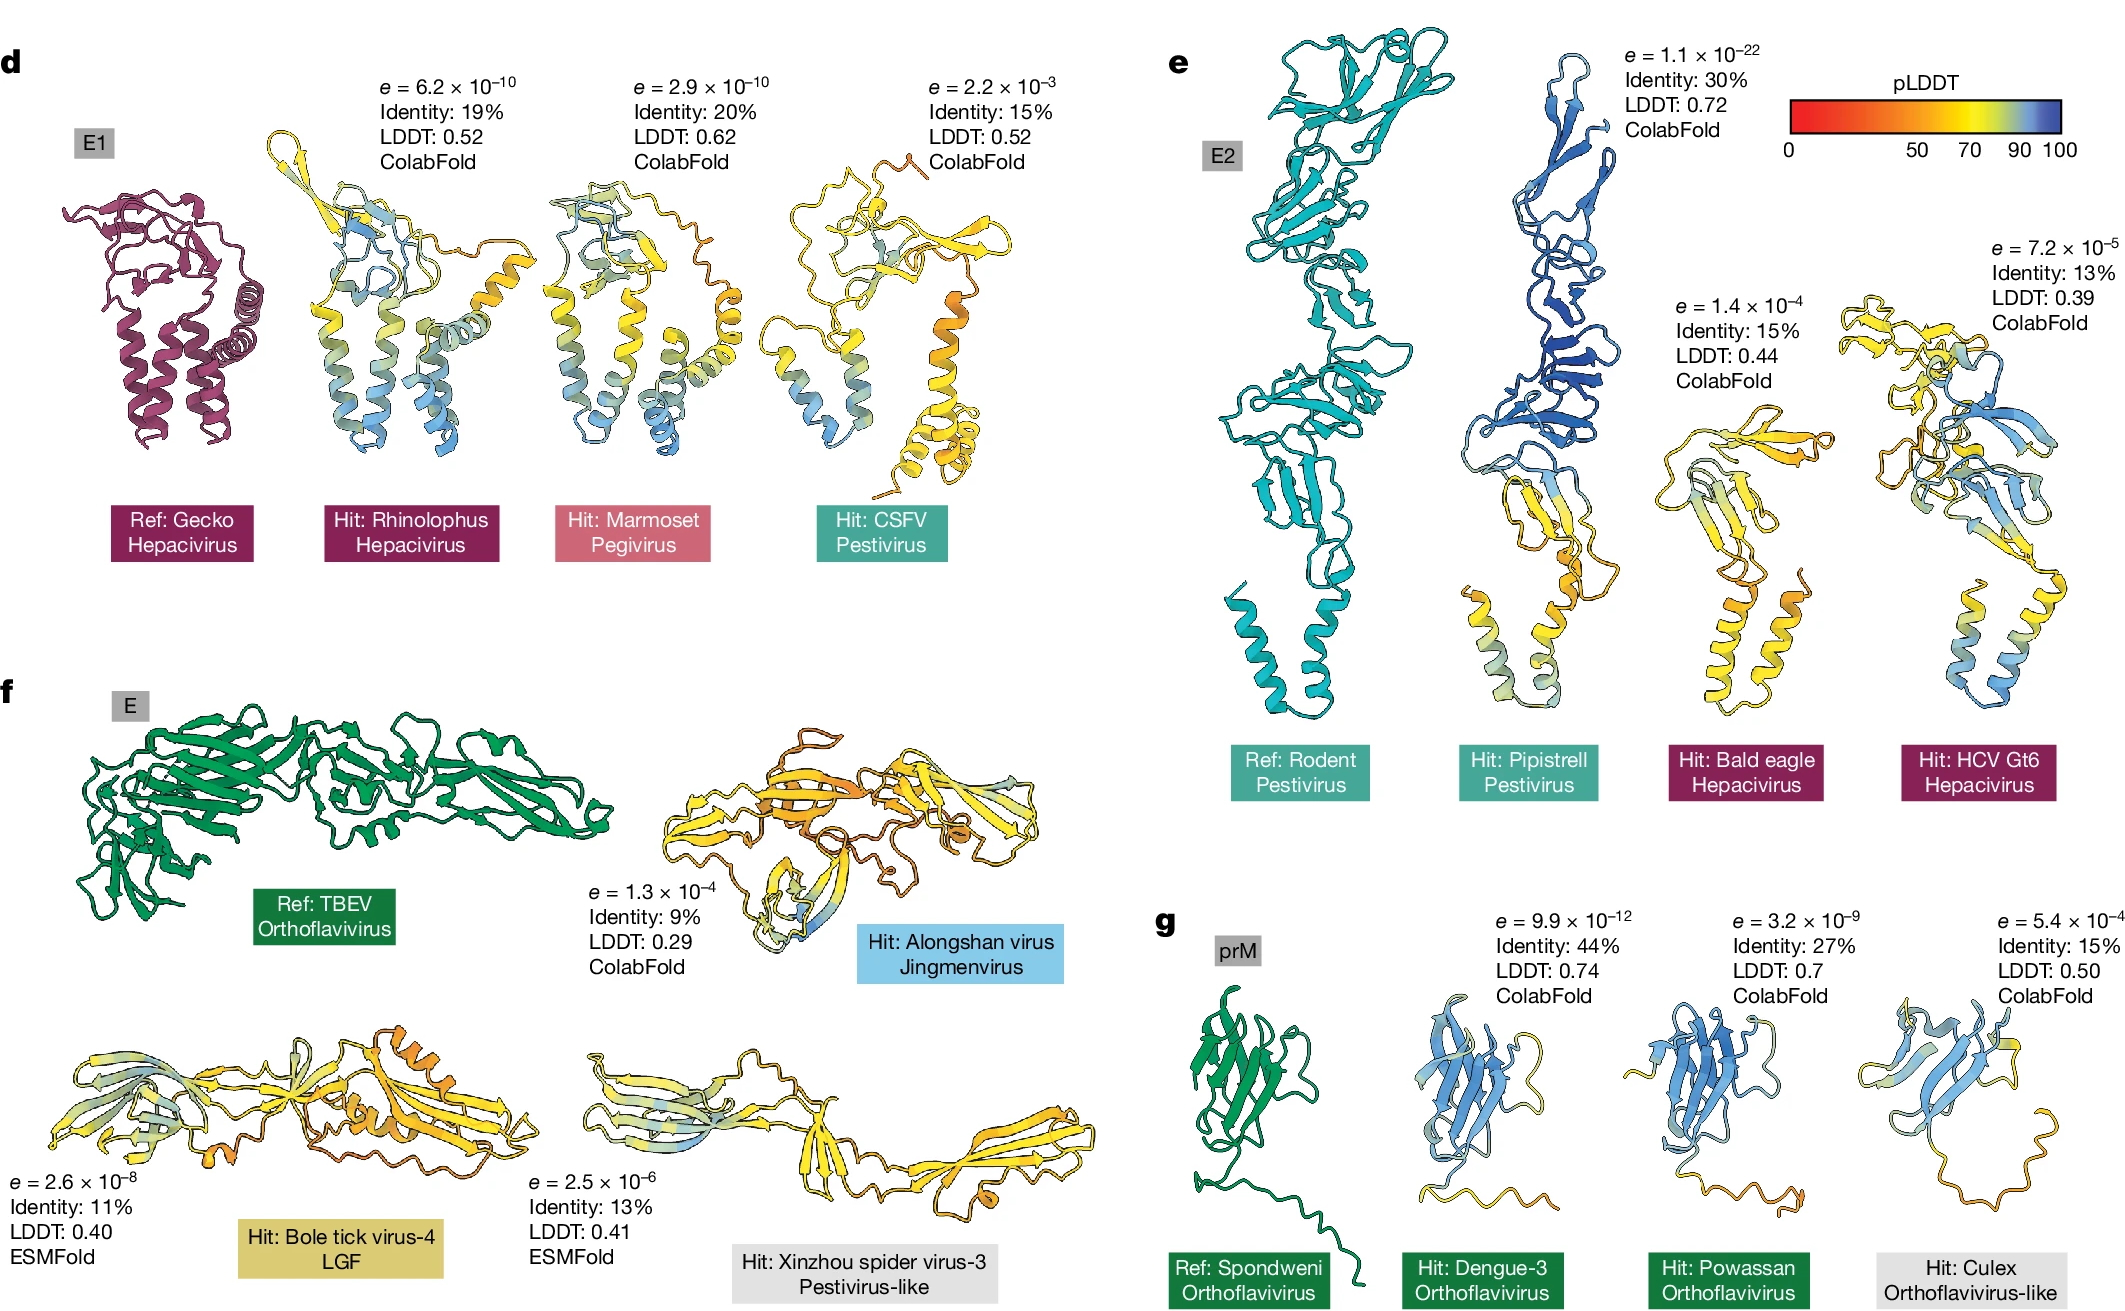
\includegraphics[width=.9\textwidth]{/workspaces/seminar-bioinformatik/images/figure2.jpg}
    \caption{Illustration der pLDDT-Werte in Korrelation mit den \gls{msa}-Alignments}
    \label{fig:figure2-orginal}
\end{figure}

Die Abbildung zeigt die Korrelation zwischen den pLDDT-Werten und den \gls{msa}-Alignments. Die Farbskala repräsentiert die Zuverlässigkeit der Strukturvorhersagen, wobei hohe pLDDT-Werte (blau) auf eine hohe Übereinstimmung mit den Alignments hinweisen. Die Analyse der pLDDT-Werte ermöglicht eine präzise Bewertung der Strukturqualität und Identifikation von konservierten Regionen innerhalb der Glycoproteine.

\section{Homologiesuche: Anwendung von Foldseek} \label{sec:foldseek}

Zur Identifizierung struktureller Homologien zwischen den vorhergesagten Glycoprotein-Strukturen wurde das Programm \gls{foldseek} eingesetzt \autocite{vankempenFastAccurateProtein2024}. Foldseek ermöglicht einen schnellen Vergleich von Proteinstrukturen, indem es deren dreidimensionale Koordinaten in vereinfachte Merkmalsrepräsentationen umwandelt. Diese Methode ist besonders effizient, um strukturelle Ähnlichkeiten auch bei hoher Sequenzdivergenz zu erkennen, was klassische sequenzbasierte Methoden wie BLAST nicht leisten können \autocite{Altschul1990}.

Die vorhergesagten Glycoprotein-Strukturen aus \gls{colabfold} und \gls{esmfold} wurden mit bekannten Strukturen aus der Protein Data Bank (\gls{pdb}) verglichen. Die Übereinstimmung der Modelle wurde durch Alignment-Scores und \gls{rmsd}-Werte quantifiziert, deren mathematische Grundlagen im Anhang \ref{sec:rmsd-berechnung} erläutert werden. Konservierte Faltungsmuster und potenzielle funktionelle Gemeinsamkeiten, wie die Klasse-II-Fusionsproteinfaltung, wurden identifiziert.

Die Ergebnisse der Homologiesuche wurden anschließend mit den phylogenetischen Analysen kombiniert, um divergente und konvergente evolutionäre Anpassungen innerhalb der Flaviviridae zu identifizieren. Auf diese Weise konnten strukturelle Gemeinsamkeiten zwischen verschiedenen Gattungen trotz erheblicher Sequenzunterschiede nachgewiesen werden.